\documentclass[aspectratio=169]{beamer}
\usepackage[utf8]{inputenc}\usepackage[T1]{fontenc}\usepackage{lmodern}
\usetheme{Madrid}
\setbeamertemplate{navigation symbols}{}
\setbeamercovered{transparent}
\setbeamertemplate{itemize items}[circle]
\setbeamertemplate{enumerate items}[default]
\setlength{\parskip}{0.25em}
\definecolor{UNBCDark}{RGB}{0,74,37}
\definecolor{UNBCGold}{RGB}{189,155,96}
\definecolor{SoftGray}{RGB}{244,246,248}
\definecolor{AccentRed}{RGB}{192,57,43}
\definecolor{AccentBlue}{RGB}{41,98,255}
\definecolor{AccentTeal}{RGB}{0,150,136}
\definecolor{AccentOrange}{RGB}{230,126,34}
\setbeamercolor{normal text}{fg=black,bg=white}
\setbeamercolor{structure}{fg=UNBCDark}
\setbeamercolor{title}{fg=white,bg=UNBCDark}
\setbeamercolor{subtitle}{fg=UNBCGold}
\setbeamercolor{frametitle}{fg=white,bg=UNBCDark}
\setbeamercolor{block title}{fg=white,bg=UNBCDark}
\setbeamercolor{block body}{fg=black,bg=SoftGray}
\setbeamercolor{block title alerted}{fg=white,bg=AccentRed}
\setbeamercolor{block body alerted}{fg=black,bg=SoftGray}
\setbeamercolor{item}{fg=UNBCDark}
\setbeamercolor{alerted text}{fg=AccentRed}
\setbeamercolor{author in head/foot}{fg=white,bg=UNBCDark}
\setbeamercolor{date in head/foot}{fg=white,bg=UNBCDark}
\usepackage{booktabs,multirow,array,amsmath,amssymb,bm,graphicx,adjustbox}
\usepackage{tikz,pgfplots,multicol,tcolorbox,hyperref}
\tcbuselibrary{skins}
\pgfplotsset{compat=1.18}
\usetikzlibrary{arrows.meta,positioning,calc,decorations.pathreplacing}
\hypersetup{colorlinks=true,linkcolor=UNBCDark}
\setbeamertemplate{headline}{}
\setbeamertemplate{footline}{%
  \leavevmode\hbox{%
  \begin{beamercolorbox}[wd=.78\paperwidth,ht=2.8ex,dp=1.2ex,leftskip=1em]{author in head/foot}%
  \color{white}\textbf{ECON 308} \hspace{0.4em}\textcolor{UNBCGold}{|}\hspace{0.4em}International Economic Relations%
  \end{beamercolorbox}%
  \begin{beamercolorbox}[wd=.22\paperwidth,ht=2.8ex,dp=1.2ex,rightskip=1em plus1fil]{date in head/foot}%
  \color{white}\insertframenumber/\inserttotalframenumber%
  \end{beamercolorbox}}%
}
\newtcolorbox{insight}[1]{colback=UNBCGold!12,colframe=UNBCGold!70!black,
  title={\small\bfseries #1},left=1.5mm,right=1.5mm,top=0.8mm,bottom=0.8mm,boxrule=0.5pt,arc=2mm}
\newtcolorbox{canadex}[1][Canadian Example]{colback=AccentTeal!9,colframe=AccentTeal,
  title={\small\bfseries #1},left=1.5mm,right=1.5mm,top=0.8mm,bottom=0.8mm,boxrule=0.5pt,arc=2mm}
\newtcolorbox{discuss}{colback=AccentBlue!8,colframe=AccentBlue,
  title={\small\bfseries Discussion},left=1.5mm,right=1.5mm,top=0.8mm,bottom=0.8mm,boxrule=0.5pt,arc=2mm}
\newtcolorbox{varbox}{colback=SoftGray,colframe=UNBCDark!50,
  left=1.5mm,right=1.5mm,top=0.8mm,bottom=0.8mm,boxrule=0.4pt,arc=2mm}
\newcommand{\FIG}[1]{\begin{center}%
  \includegraphics[width=\textwidth,height=0.68\textheight,keepaspectratio]{#1}%
  \end{center}}
\newcommand{\FIGH}[2][0.85]{\begin{center}%
  \includegraphics[width=#1\textwidth,height=0.72\textheight,keepaspectratio]{#2}%
  \end{center}}

\title{\textbf{The Standard Trade Model}}
\subtitle{{\large ECON 308 -- International Economic Relations \quad Chapter 6}}
\author{Muhebullah Karimzada}
\institute{School of Economics \\ University of Northern British Columbia}
\date{Fall 2026}

\begin{document}

\begin{frame}[plain]\titlepage\end{frame}

\begin{frame}{The Standard Model: A Unified Framework}
\begin{columns}
\begin{column}{0.57\textwidth}
\begin{itemize}
  \item The Ricardian model has a straight-line PPF (one factor).
  \item The H-O model has a bowed-out PPF (two factors).
  \item The \textbf{standard trade model} works with any bowed-out PPF --- it nests both as special cases and allows us to answer:
    \begin{enumerate}
      \item How do changes in the \emph{terms of trade} affect welfare?
      \item How does \emph{economic growth} affect trade and welfare?
      \item When can a country benefit from imposing a tariff?
    \end{enumerate}
\end{itemize}
\end{column}
\begin{column}{0.40\textwidth}
\begin{insight}{Why This Matters}
  The standard model provides the clearest framework for understanding how changes in \emph{world prices} affect national welfare --- a key question for Canada as a commodity exporter.
\end{insight}
\end{column}
\end{columns}
\end{frame}

\begin{frame}{Learning Objectives}
\begin{enumerate}
  \item Define the terms of trade and explain why they determine welfare.
  \item Use the standard model to analyse growth and its effects on the ToT.
  \item Distinguish export-biased from import-biased growth.
  \item Explain the conditions for immiserising growth.
  \item Analyse how tariffs and export subsidies affect the terms of trade and welfare.
  \item Apply these concepts to Canadian trade policy debates.
\end{enumerate}
\end{frame}

\begin{frame}{The Production Possibility Frontier (Bowed-Out)}
\begin{columns}
\begin{column}{0.5\textwidth}
\textbf{Why bowed-out?}\\
With multiple factors, increasing production of cloth requires pulling factors that are progressively less suited for it (more capital-intensive workers, land not suited for textile mills).\\[0.3em]
\textbf{Opportunity cost of cloth rises} as cloth output rises.\\[0.4em]
\textbf{Production equilibrium:} the economy produces where the \textbf{isovalue line} is tangent to the PPF:
\[P_C \cdot Q_C + P_F \cdot Q_F = \text{maximised}\]
The slope of the isovalue line = $-P_C/P_F$.
\end{column}
\begin{column}{0.47\textwidth}
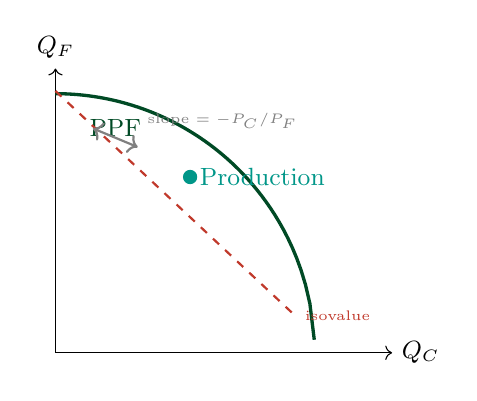
\begin{tikzpicture}[scale=0.95]
\draw[->] (0,0) -- (4.5,0) node[right]{\small $Q_C$};
\draw[->] (0,0) -- (0,3.8) node[above]{\small $Q_F$};
\draw[UNBCDark,very thick,domain=0:3.46,samples=60] plot(\x,{sqrt(max(0,12-\x*\x))});
\node[UNBCDark] at (0.8,3) {\small PPF};
\draw[AccentRed,thick,dashed] (0,3.5) -- (3.2,0.5) node[right]{\tiny isovalue};
\filldraw[AccentTeal] (1.8,2.35) circle(2.5pt) node[right]{\small Production};
\draw[<->,gray,thick] (0.5,3.0) -- (1.1,2.75);
\node[gray,right] at (1.1,3.1) {\tiny slope $= -P_C/P_F$};
\end{tikzpicture}
\end{column}
\end{columns}
\end{frame}

\begin{frame}{Consumption Choices and Social Indifference Curves}
\begin{columns}
\begin{column}{0.5\textwidth}
\textbf{Consumption equilibrium:} maximise social welfare $U(D_C, D_F)$ subject to the budget constraint:
\[P_C \cdot D_C + P_F \cdot D_F = P_C \cdot Q_C + P_F \cdot Q_F\]
where $D_C, D_F$ are consumption of cloth and food.\\[0.4em]
\textbf{Key}: under trade, the budget line has slope $-P_C/P_F$ (world prices) and passes through the \emph{production} point.\\[0.3em]
Consumption can be \textbf{anywhere on the budget line} --- not just on the PPF.
\end{column}
\begin{column}{0.47\textwidth}
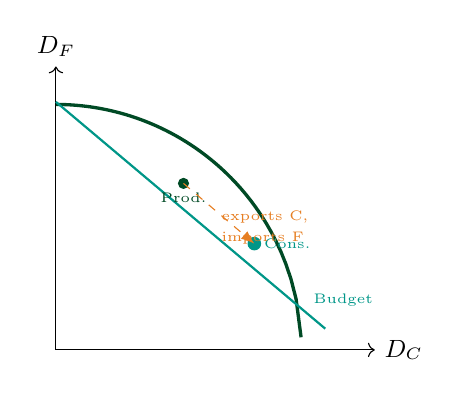
\begin{tikzpicture}[scale=0.9]
\draw[->] (0,0) -- (4.5,0) node[right]{\small $D_C$};
\draw[->] (0,0) -- (0,4) node[above]{\small $D_F$};
% PPF
\draw[UNBCDark,very thick,domain=0:3.46,samples=50] plot(\x,{sqrt(max(0,12-\x*\x))});
% Budget line
\draw[AccentTeal,thick] (0,3.5) -- (3.8,0.3);
\node[AccentTeal,right] at (3.5,0.7) {\tiny Budget};
% Production point
\filldraw[UNBCDark] (1.8,2.35) circle(2pt) node[below]{\tiny Prod.};
% Consumption point (off PPF)
\filldraw[AccentTeal] (2.8,1.5) circle(2.5pt) node[right]{\tiny Cons.};
% Difference = imports/exports
\draw[-{Latex},AccentOrange,dashed] (1.8,2.35) -- (2.8,1.5);
\node[AccentOrange,below right] at (2.2,2.1) {\tiny exports C,};
\node[AccentOrange,below right] at (2.2,1.8) {\tiny imports F};
\end{tikzpicture}
\end{column}
\end{columns}
\end{frame}

\begin{frame}{Terms of Trade: Definition and Welfare Link}
\begin{block}{Definition}
The \textbf{terms of trade (ToT)} for a country = price of its \emph{exports} divided by price of its \emph{imports}:
\[\text{ToT} = \frac{P_{\text{export}}}{P_{\text{import}}}\]
For Home (cloth exporter): $\text{ToT} = P_C/P_F$.
\end{block}
\vspace{0.3em}
\begin{columns}
\begin{column}{0.52\textwidth}
\textbf{Welfare and the ToT:}
\begin{itemize}
  \item ToT $\uparrow$ (export prices rise): budget line rotates outward $\Rightarrow$ higher CIC $\Rightarrow$ welfare \textbf{rises}.
  \item ToT $\downarrow$ (import prices rise): budget line rotates inward $\Rightarrow$ lower CIC $\Rightarrow$ welfare \textbf{falls}.
  \item The ToT is the single most important price variable for a small open economy's welfare.
\end{itemize}
\end{column}
\begin{column}{0.45\textwidth}
\begin{canadex}[Canada's ToT 1990--2020]
  Oil price: $\sim$\$20 (1990) $\to$ \$110 (2014) $\to$ \$45 (2016) $\to$ \$85 (2023).\\[0.3em]
  Canada's ToT closely tracks oil prices. The 1990--2014 improvement added $\sim$15\% to real national income \emph{beyond} real GDP growth.
\end{canadex}
\end{column}
\end{columns}
\end{frame}

\begin{frame}{Figure 6-8: Evolution of US Terms of Trade}
\begin{columns}
\begin{column}{0.54\textwidth}
\FIGH[0.96]{figures/slide34_img01.PNG}
\end{column}
\begin{column}{0.43\textwidth}
\textbf{Reading Figure 6-8:}
\begin{itemize}\small
  \item \textbf{Vertical axis}: US terms of trade index (export prices / import prices), normalised to 100 in some base year.
  \item \textbf{Long-run trend}: relatively stable with cyclical swings driven by energy prices.
  \item \textbf{Oil shocks}: 1973, 1979 oil price spikes worsened US ToT (US imports oil).
  \item \textbf{Post-2008}: shale revolution reduced US oil imports, improving ToT.
  \item The US is a large economy --- its growth and policies \emph{affect} world prices (and hence its own ToT).
\end{itemize}
\begin{insight}{Contrast with Canada}
  Canada is an oil exporter --- its ToT moves \emph{opposite} to the US when oil prices change.
\end{insight}
\end{column}
\end{columns}
\end{frame}

\begin{frame}{World Relative Supply and Demand}
\begin{columns}
\begin{column}{0.5\textwidth}
\textbf{World Relative Supply (RS):} upward-sloping.\\
Higher $P_C/P_F$ induces both countries to shift production toward cloth $\Rightarrow$ world relative supply of cloth rises.\\[0.4em]
\textbf{World Relative Demand (RD):} downward-sloping.\\
Higher $P_C/P_F$ induces consumers worldwide to substitute toward food $\Rightarrow$ relative demand for cloth falls.\\[0.4em]
\textbf{World equilibrium:} RS = RD determines $p^* = P_C^*/P_F^*$.\\[0.3em]
Shifts in either curve change the equilibrium ToT.
\end{column}
\begin{column}{0.47\textwidth}
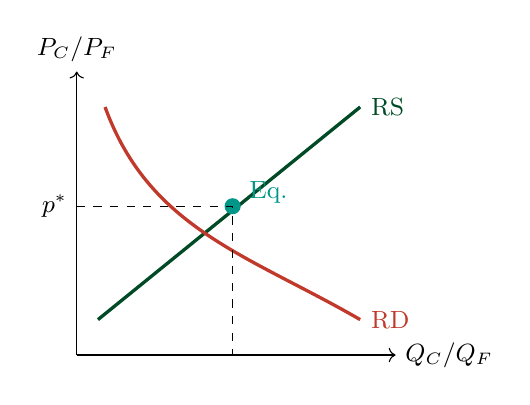
\begin{tikzpicture}[scale=0.9]
\draw[->] (0,0) -- (4.5,0) node[right]{\small $Q_C/Q_F$};
\draw[->] (0,0) -- (0,4) node[above]{\small $P_C/P_F$};
\draw[UNBCDark,very thick] (0.3,0.5) -- (4,3.5) node[right]{\small RS};
\draw[AccentRed,very thick] (0.4,3.5) to[out=-70,in=150] (4,0.5) node[right]{\small RD};
\filldraw[AccentTeal] (2.2,2.1) circle(3pt);
\draw[dashed] (0,2.1) node[left]{\small $p^*$} -- (2.2,2.1) -- (2.2,0);
\node[AccentTeal,right] at (2.3,2.3) {\small Eq.};
\end{tikzpicture}
\end{column}
\end{columns}
\end{frame}

\begin{frame}{Economic Growth: Export-Biased vs.\ Import-Biased}
\begin{block}{Growth Bias}
\textbf{Export-biased growth}: expands production of the export good (cloth) more than the import good (food) at constant prices. RS shifts right $\Rightarrow$ ToT \textbf{deteriorates}.\\[0.3em]
\textbf{Import-biased growth}: expands production of the import good more, or raises demand for imports (biased consumption). ToT also \textbf{deteriorates}.
\end{block}
\vspace{0.3em}
\begin{columns}
\begin{column}{0.52\textwidth}
\textbf{Export-biased growth} (Rybczynski):
\begin{itemize}
  \item Growth in factor used intensively in export good.
  \item More cloth produced at given prices.
  \item World price of cloth falls: ToT worsen.
\end{itemize}
\end{column}
\begin{column}{0.45\textwidth}
\begin{canadex}[China's Impact on Canada]
  China's rapid growth (import-biased from Canada's perspective) \emph{increased} demand for Canadian commodities. Canada's ToT improved 2002--2014 as China bought more oil, potash, lumber, and copper. Canada benefited from China's growth.
\end{canadex}
\end{column}
\end{columns}
\end{frame}

\begin{frame}{Immiserising Growth: When Growth Makes You Poorer}
\begin{block}{Bhagwati (1958): Immiserising Growth}
A country can be made \textbf{worse off by economic growth} if:
\begin{enumerate}
  \item Growth is \emph{strongly export-biased} (Rybczynski).
  \item The country is \emph{large} enough to affect world prices.
  \item World demand for its export is \emph{price-inelastic}.
\end{enumerate}
Then: ToT deterioration \emph{exceeds} the direct production gain $\Rightarrow$ net welfare loss.
\end{block}
\vspace{0.3em}
\begin{columns}
\begin{column}{0.52\textwidth}
\textbf{Conditions for immiserising growth:}
\begin{itemize}
  \item Large-country effects: more growth worsens ToT more.
  \item Inelastic demand: price falls a lot when supply rises.
  \item Strong bias: growth concentrated in export sector.
\end{itemize}
\textbf{Prebisch-Singer hypothesis}: commodity exporters face long-run secular ToT deterioration --- a possible immiserising growth trap.
\end{column}
\begin{column}{0.45\textwidth}
\begin{canadex}
  BC \emph{dramatically} increases timber harvesting. Global lumber price falls sharply. Revenue may actually \emph{fall} even as output rises.\\[0.3em]
  This is why sustainable forestry quotas can actually \emph{increase} BC's forestry revenue by keeping prices high.
\end{canadex}
\end{column}
\end{columns}
\end{frame}

\begin{frame}{Tariffs and the Terms of Trade}
\begin{columns}
\begin{column}{0.52\textwidth}
\textbf{Large-country tariff on food imports:}
\begin{enumerate}
  \item Tariff reduces Home's demand for food imports.
  \item World price of food \textbf{falls} (foreign exporters sell less).
  \item Home's ToT improve: each unit of cloth now buys more food.
  \item But: tariff creates domestic deadweight losses.
\end{enumerate}
\vspace{0.3em}
\textbf{Net welfare effect:}\\
ToT gain $-$ domestic efficiency loss.\\
If country is large enough and ToT gain dominates: \textbf{optimal tariff} is positive.
\end{column}
\begin{column}{0.45\textwidth}
\begin{alertblock}{The Trade War Risk}
  The optimal tariff argument is valid for one country in isolation. But if all countries impose optimal tariffs, a \emph{trade war} erupts. The Nash equilibrium (mutual protection) leaves \emph{all countries worse off} than mutual free trade.\\[0.3em]
  This is the prisoner's dilemma of trade policy --- solved by GATT/WTO commitments.
\end{alertblock}
\end{column}
\end{columns}
\end{frame}

\begin{frame}{Export Subsidies and the Terms of Trade}
\begin{columns}
\begin{column}{0.52\textwidth}
\textbf{Export subsidy} on cloth:
\begin{itemize}
  \item Government pays domestic cloth producers per unit exported.
  \item More cloth flows to world market $\Rightarrow$ world price of cloth falls.
  \item Home's ToT \textbf{deteriorate} (export price falls).
  \item \textbf{Result}: Home consumers pay more for cloth; Home government pays the subsidy; ToT worsen.
\end{itemize}
\vspace{0.2em}
\textbf{Export subsidies are worse than tariffs} for the subsidising country: both create domestic distortions but subsidies \emph{also} worsen the ToT.
\end{column}
\begin{column}{0.45\textwidth}
\begin{canadex}[EU Agricultural Export Subsidies]
  The EU's Common Agricultural Policy paid billions in export subsidies on wheat and dairy through the 1990s.\\[0.3em]
  This dumped cheap food on world markets, hurting farmers in developing countries and worsening EU ToT.\\[0.3em]
  Under WTO pressure (Doha Round), EU agreed to phase out export subsidies. Fully eliminated by 2013.
\end{canadex}
\end{column}
\end{columns}
\end{frame}

\begin{frame}{Key Takeaways}
\begin{enumerate}
  \item The standard trade model uses bowed-out PPFs and social indifference curves to analyse welfare.
  \item \textbf{Terms of trade} are the key welfare variable: ToT improvement raises welfare; deterioration lowers it.
  \item \textbf{Export-biased growth} worsens a country's ToT; \textbf{import-biased growth} in trading partners can improve your ToT.
  \item \textbf{Immiserising growth} is possible if growth is export-biased, the country is large, and world demand is inelastic.
  \item \textbf{Large-country tariff} improves ToT but invites retaliation --- trade wars hurt all.
  \item \textbf{Export subsidies} are even worse: they simultaneously distort the domestic economy and worsen the ToT.
\end{enumerate}
\begin{block}{Next: Chapter 7 --- Economies of Scale and Trade}
  Why do similar countries trade similar goods? Intra-industry trade and the Krugman model.
\end{block}
\end{frame}

\end{document}
